\documentclass[tikz, convert=pdf2svg]{standalone}
\usetikzlibrary{positioning}
\begin{document}
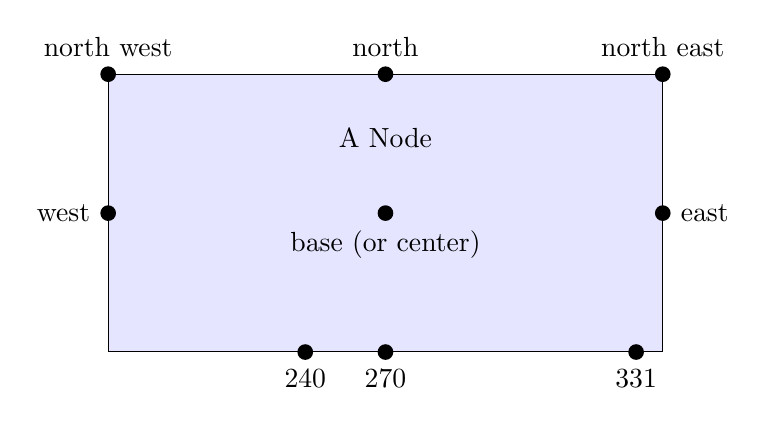
\begin{tikzpicture}
    \node[draw, minimum width=200pt, minimum height=100pt, fill=blue!10, label={[yshift=-30pt]A Node}] (anchor) {};

    \node[circle, fill=black, inner sep=2pt] at (anchor.north) {} node[above=3pt of anchor.north] {north};
    \node[circle, fill=black, inner sep=2pt] at (anchor.north east) {} node[above=3pt of anchor.north east] {north east};
    \node[circle, fill=black, inner sep=2pt] at (anchor.north west) {} node[above=3pt of anchor.north west] {north west};
    \node[circle, fill=black, inner sep=2pt] at (anchor.west) {} node[left=3pt of anchor.west] {west};
    \node[circle, fill=black, inner sep=2pt] at (anchor.east) {} node[right=3pt of anchor.east] {east};
    \node[circle, fill=black, inner sep=2pt] at (anchor.240) {} node[below=3pt of anchor.240] {240};
    \node[circle, fill=black, inner sep=2pt] at (anchor.270) {} node[below=3pt of anchor.270] {270};
    \node[circle, fill=black, inner sep=2pt] at (anchor.331) {} node[below=3pt of anchor.331] {331};
    \node[circle, fill=black, inner sep=2pt] at (anchor.base) {} node[below=3pt of anchor.base] {base (or center)};
\end{tikzpicture}
\end{document}
